\documentclass[12pt]{article}

% Packages
\usepackage{amsmath, amssymb, mathtools}
\usepackage{graphicx}
\usepackage{physics}
\usepackage{geometry}
\usepackage{enumitem}
\usepackage{bm}
\usepackage{listings}
\usepackage{xcolor}
\usepackage{float}

% Geometry settings
\geometry{letterpaper, margin=1in}
\setlength{\parindent}{0pt}

\definecolor{codegreen}{rgb}{0,0.6,0}
\definecolor{codegray}{rgb}{0.5,0.5,0.5}
\definecolor{codepurple}{rgb}{0.58,0,0.82}
\definecolor{backcolour}{rgb}{0.95,0.95,0.92}

\lstdefinestyle{mystyle}{
    backgroundcolor=\color{backcolour},   
    commentstyle=\color{codegreen},
    keywordstyle=\color{magenta},
    numberstyle=\tiny\color{codegray},
    stringstyle=\color{codepurple},
    basicstyle=\ttfamily\footnotesize,
    breakatwhitespace=false,         
    breaklines=true,                 
    captionpos=b,                    
    keepspaces=true,                 
    numbers=left,                    
    numbersep=5pt,                  
    showspaces=false,                
    showstringspaces=false,
    showtabs=false,                  
    tabsize=2
}

\lstset{style=mystyle}

% Title
\title{ECE 148 Homework 4}
\author{Sanjot Bains}
\date{\today}

\begin{document}

\maketitle

\section*{Problem 1: Fourier Series Expansion}
The periodic signal $f(t)$ with period $T = 16$ is defined as:
\[ f(t) = \begin{cases} 
    -5, & -8 \leq t < -5 \\
    \ \ 3, & -5 \leq t < 5 \\
    -5, & \ \ 5 \leq t < 8
\end{cases} \]

\vspace{1cm}
The plot of $f(t)$ over one period is shown below:
\begin{figure}[H]
    \centering
    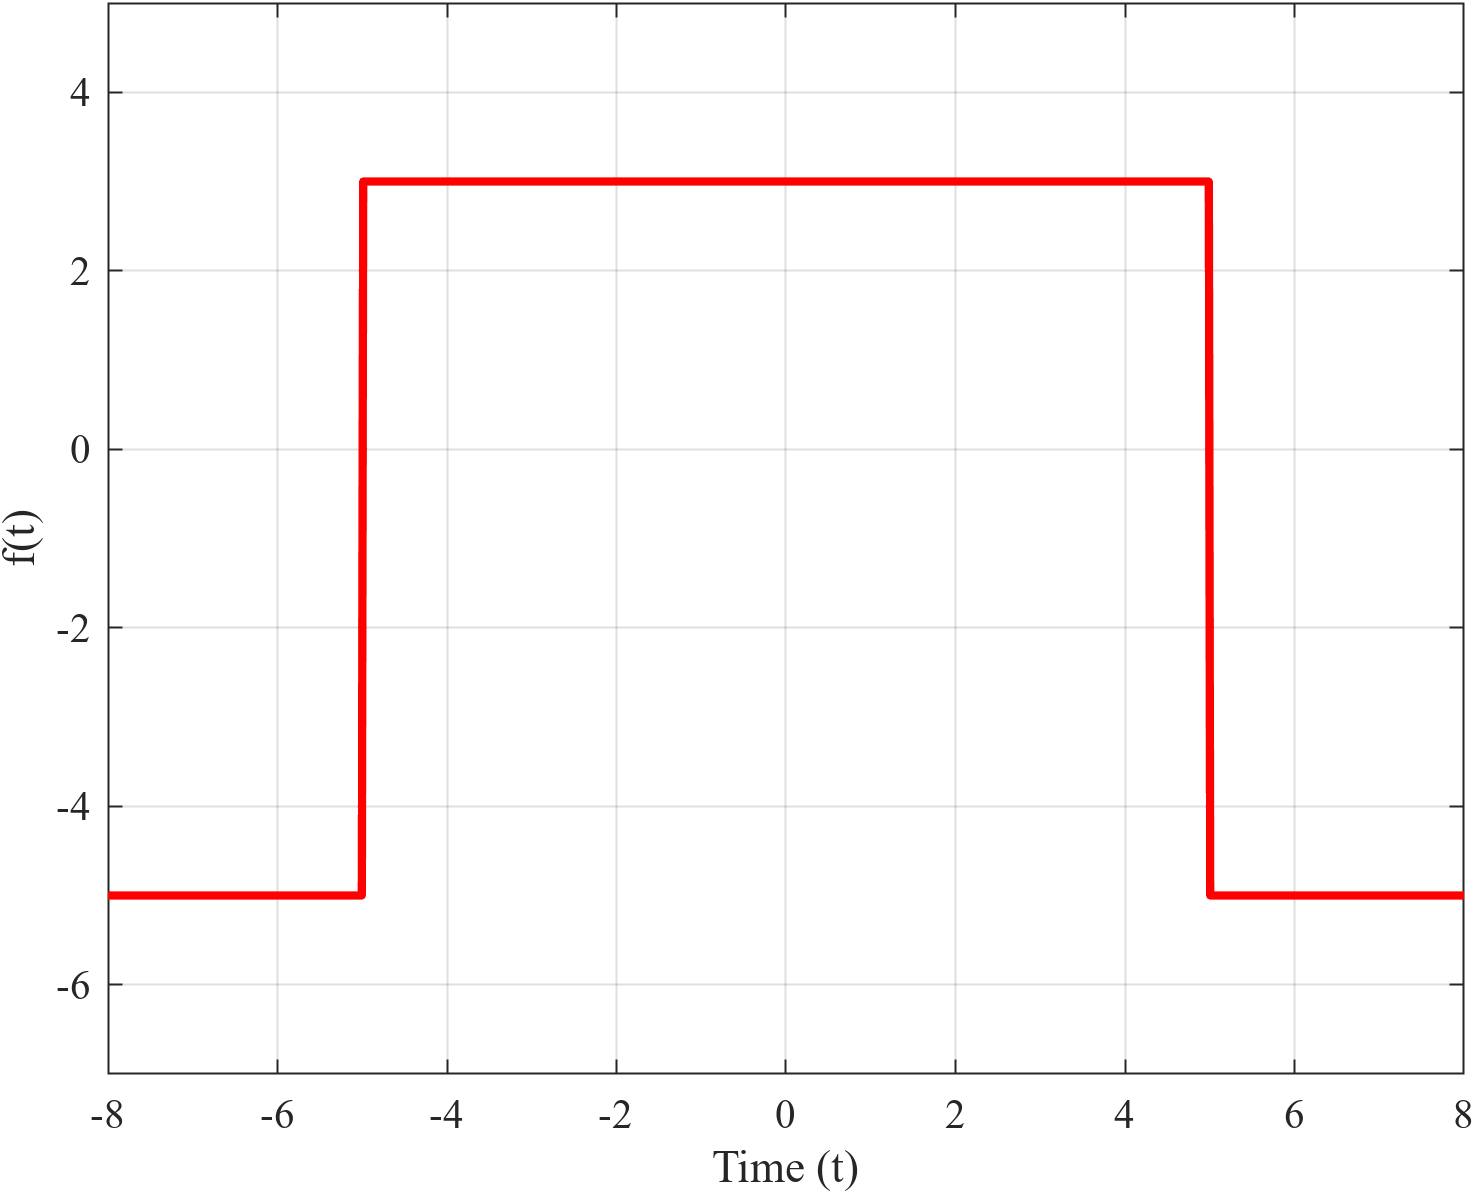
\includegraphics[width=0.8\textwidth]{f_t.png}
    \caption{Periodic Signal $f(t)$}
\end{figure}

The Fourier series expansion of $f(t)$ in complex form is given by:
\[ F_n = \frac{1}{T} \int_{-T/2}^{T/2} f(t) e^{-j n \omega_0 t} dt \]
where $\omega_0 = \frac{2\pi}{T}$ is the fundamental frequency.
Of course, in the MATLAB code we approximate the integral using a Riemann sum:
\vspace{0.25cm}
\begin{lstlisting}[language=Octave, caption=MATLAB Script to Compute Fourier Series coefficients]
w_0 = 2*pi/T;

N = 7; % Number of harmonics

k = -N:N;   

f_t = f(t);
dt = t(2) - t(1);

F_n = zeros(size(k));   
for n = 1:length(k)
    integrand = f_t .* exp(-1j * k(n) * w_0 * t);
    F_n(n) = (1/T) * sum(integrand) * dt; 
end
\end{lstlisting}


\newpage
\section*{Problem 2: Signal Reconstruction}
Using 7 harmonics ($n = \pm 1, \pm 2, \dots, \pm 7$), the signal is reconstructed as:
\[ f_{\text{reconstructed}}(t) = \sum_{n=-7}^{7} F_n e^{j n \omega_0 t} \]

\begin{lstlisting}[language=Octave, caption=MATLAB Script to Reconstruct Signal]
f_reconstructed = zeros(size(t));
for n = 1:length(k)
    f_reconstructed = f_reconstructed + F_n(n) * exp(1j * k(n) * w_0 * t);
end
\end{lstlisting}

\vspace{1cm}
The reconstructed signal is compared with the original signal below:

\begin{figure}[H]
    \centering
    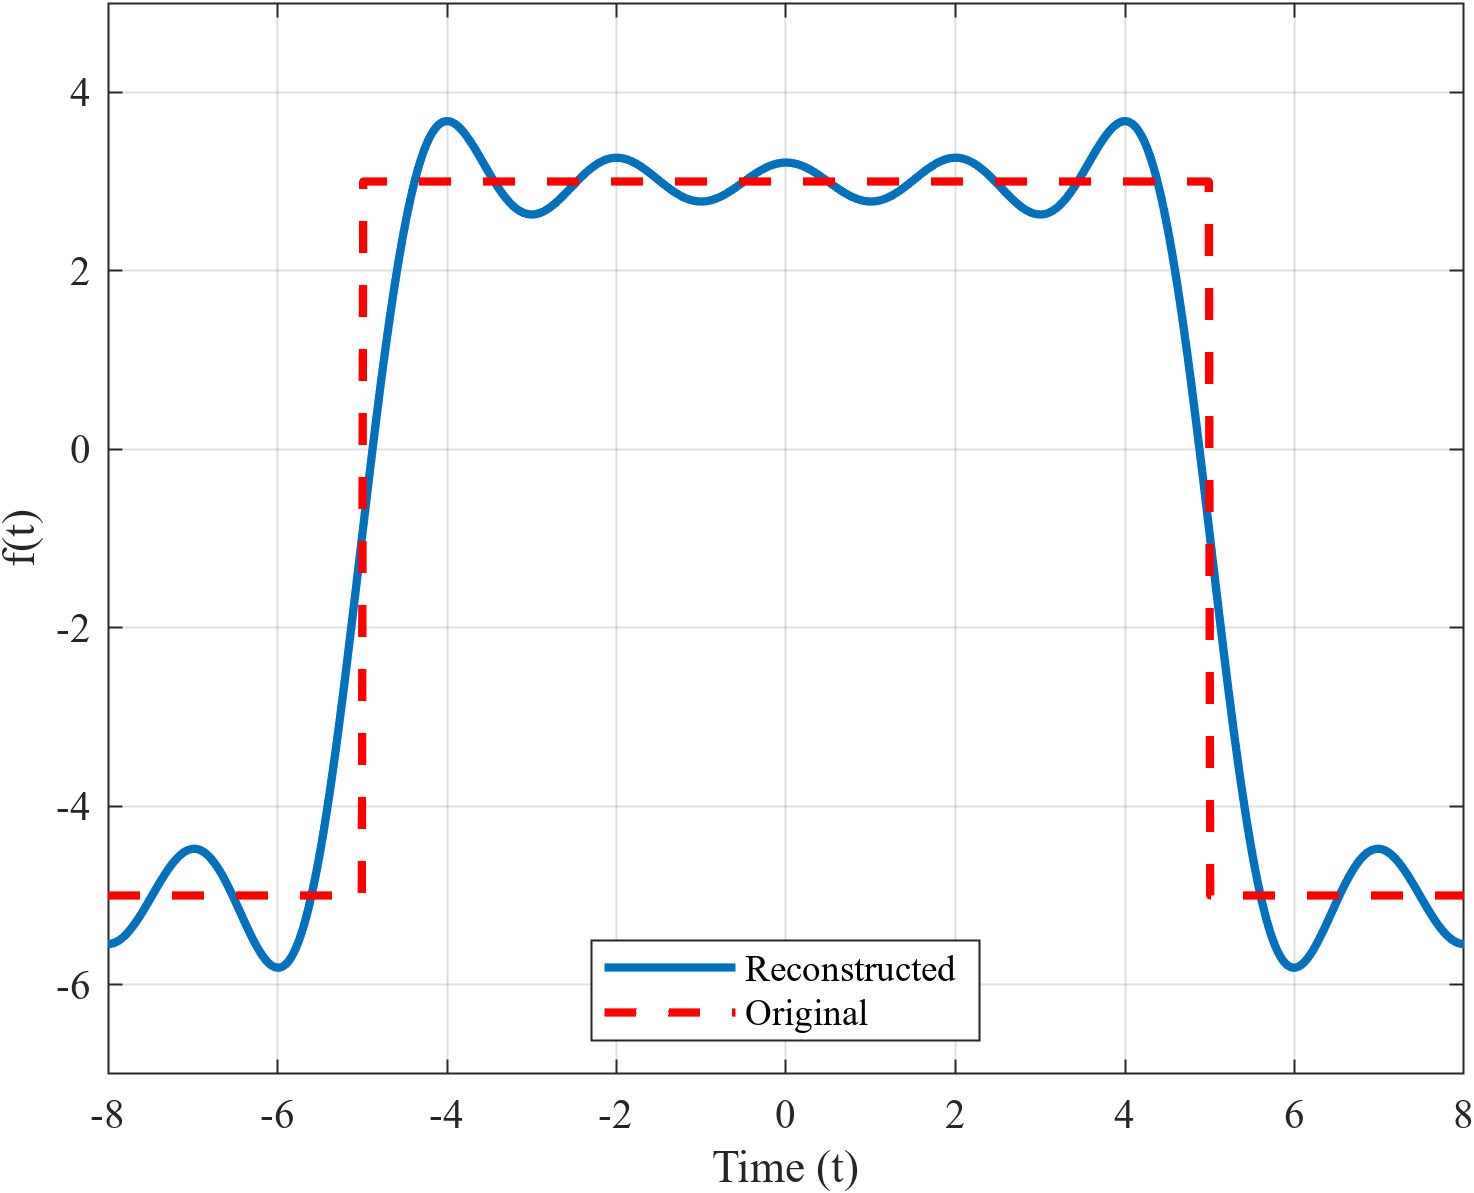
\includegraphics[width=0.8\textwidth]{f_reconstructed.png}
    \caption{Reconstructed Signal vs Original Signal}
\end{figure}


\newpage
\section*{Problem 3: DTFT of Fourier Coefficients}
The 15 Fourier coefficients $\{F_n\}$ are used to compute the DTFT:
\[ F(\omega) = \sum_{n=-7}^{7} F_n e^{-j \omega n} \]

\begin{lstlisting}[language=Octave, caption=MATLAB Script to Compute DTFT]
omega = linspace(-pi, pi, 1000);

F_omega = zeros(size(omega));
for k = 1:length(omega)
    F_omega(k) = sum(F_n .* exp(-1j * omega(k) * (-N:N)));
end
\end{lstlisting}

\vspace{1cm}
The DTFT is plotted over the interval $(-\pi, \pi)$:

\begin{figure}[H]
    \centering
    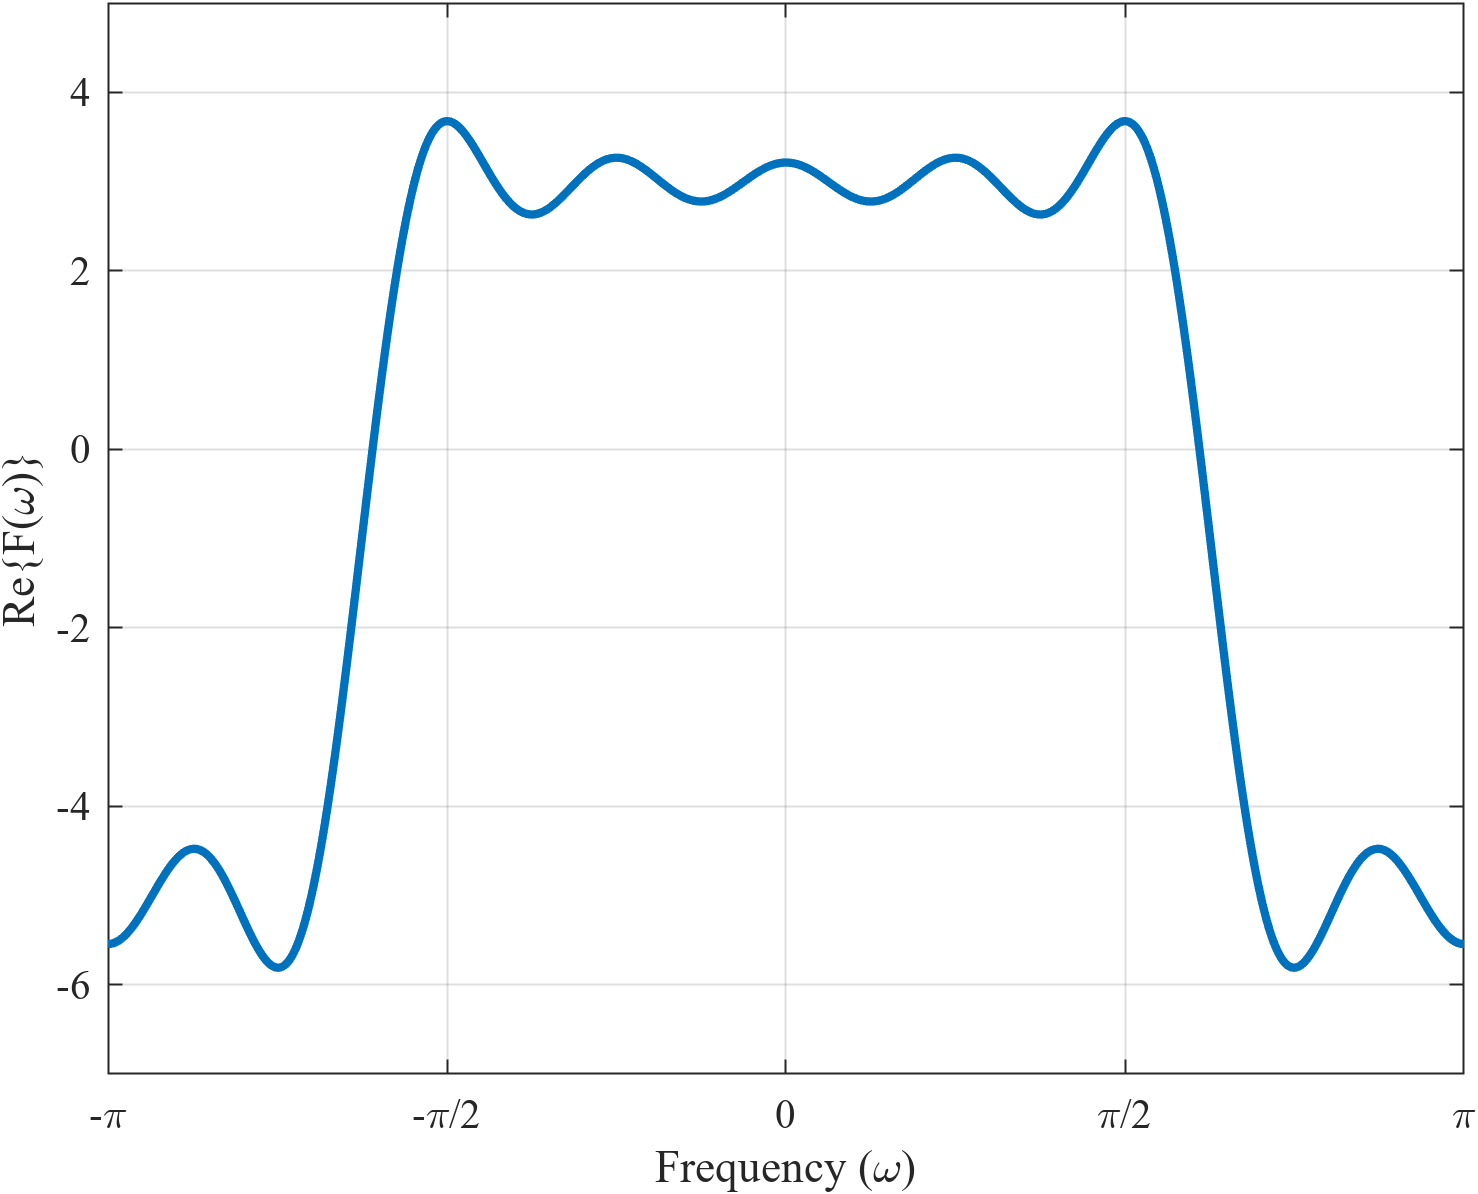
\includegraphics[width=0.8\textwidth]{DTFT.png}
    \caption{DTFT of Fourier Coefficients}
\end{figure}


\newpage
\section*{Problem 4: 32-point DFT}
The 15-point sequence $\{F_n\}$ is padded with zeros to form a 32-point sequence. The 32-point DFT is computed and plotted below:

\vspace{0.25cm}
\begin{lstlisting}[language=Octave, caption=MATLAB Script to Compute 32-point DFT]
F_32 = zeros(1, 32);
F_32(2:8) = F_n(9:15); % Positive Fourier coefficients (F_1 to F_7)
F_32(26:32) = F_n(1:7); % Negative coefficients (F_-7 to F_-1)

F_fft_32 = fft(F_32);
F_fft_32_shifted = fftshift(F_fft_32);
\end{lstlisting}

\vspace{1cm}
\begin{figure}[H]
    \centering
    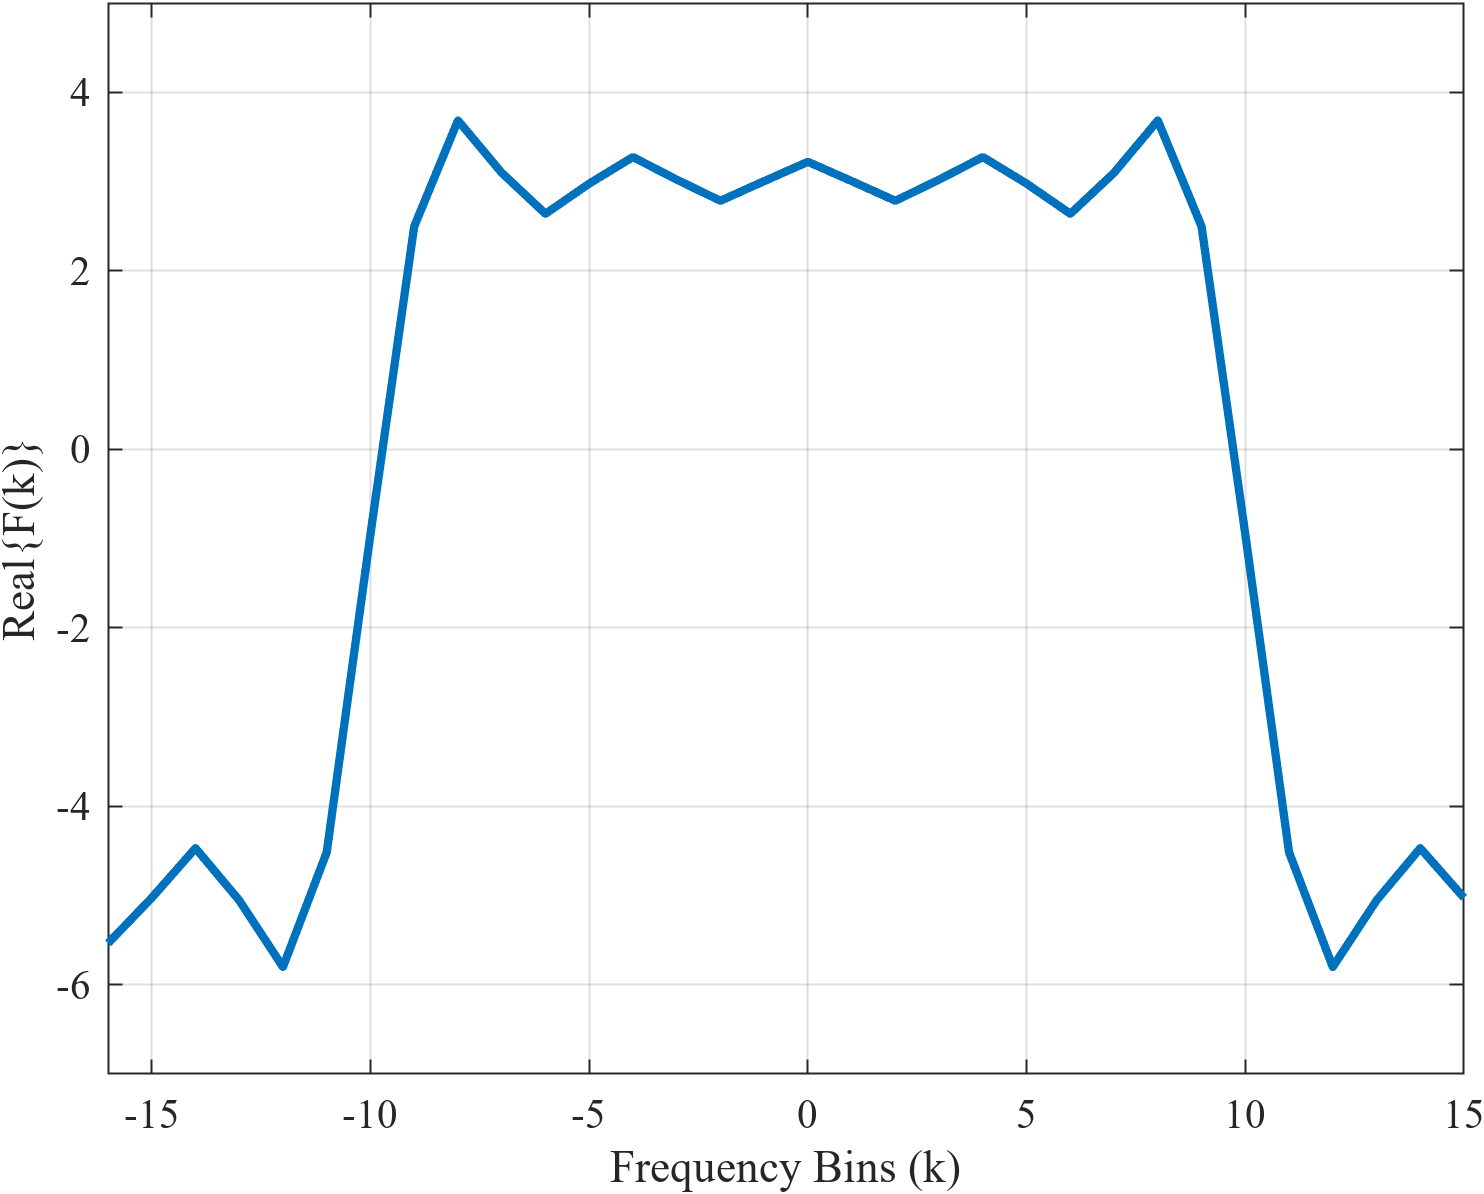
\includegraphics[width=0.8\textwidth]{DFT_32.png}
    \caption{32-point DFT of Fourier Coefficients}
\end{figure}


\newpage
\section*{Problem 5: 64-point DFT}
Similarly, the 15-point sequence $\{F_n\}$ is padded with zeros to form a 64-point sequence. The 64-point DFT is computed and plotted below:

\vspace{0.25cm}
\begin{lstlisting}[language=Octave, caption=MATLAB Script to Compute 64-point DFT]
F_64 = zeros(1, 64); 
F_64(2:8) = F_n(9:15); 
F_64(58:64) = F_n(1:7); 

F_fft_64 = fft(F_64);
F_fft_64_shifted = fftshift(F_fft_64); 
\end{lstlisting}

\vspace{1cm}
\begin{figure}[H]
    \centering
    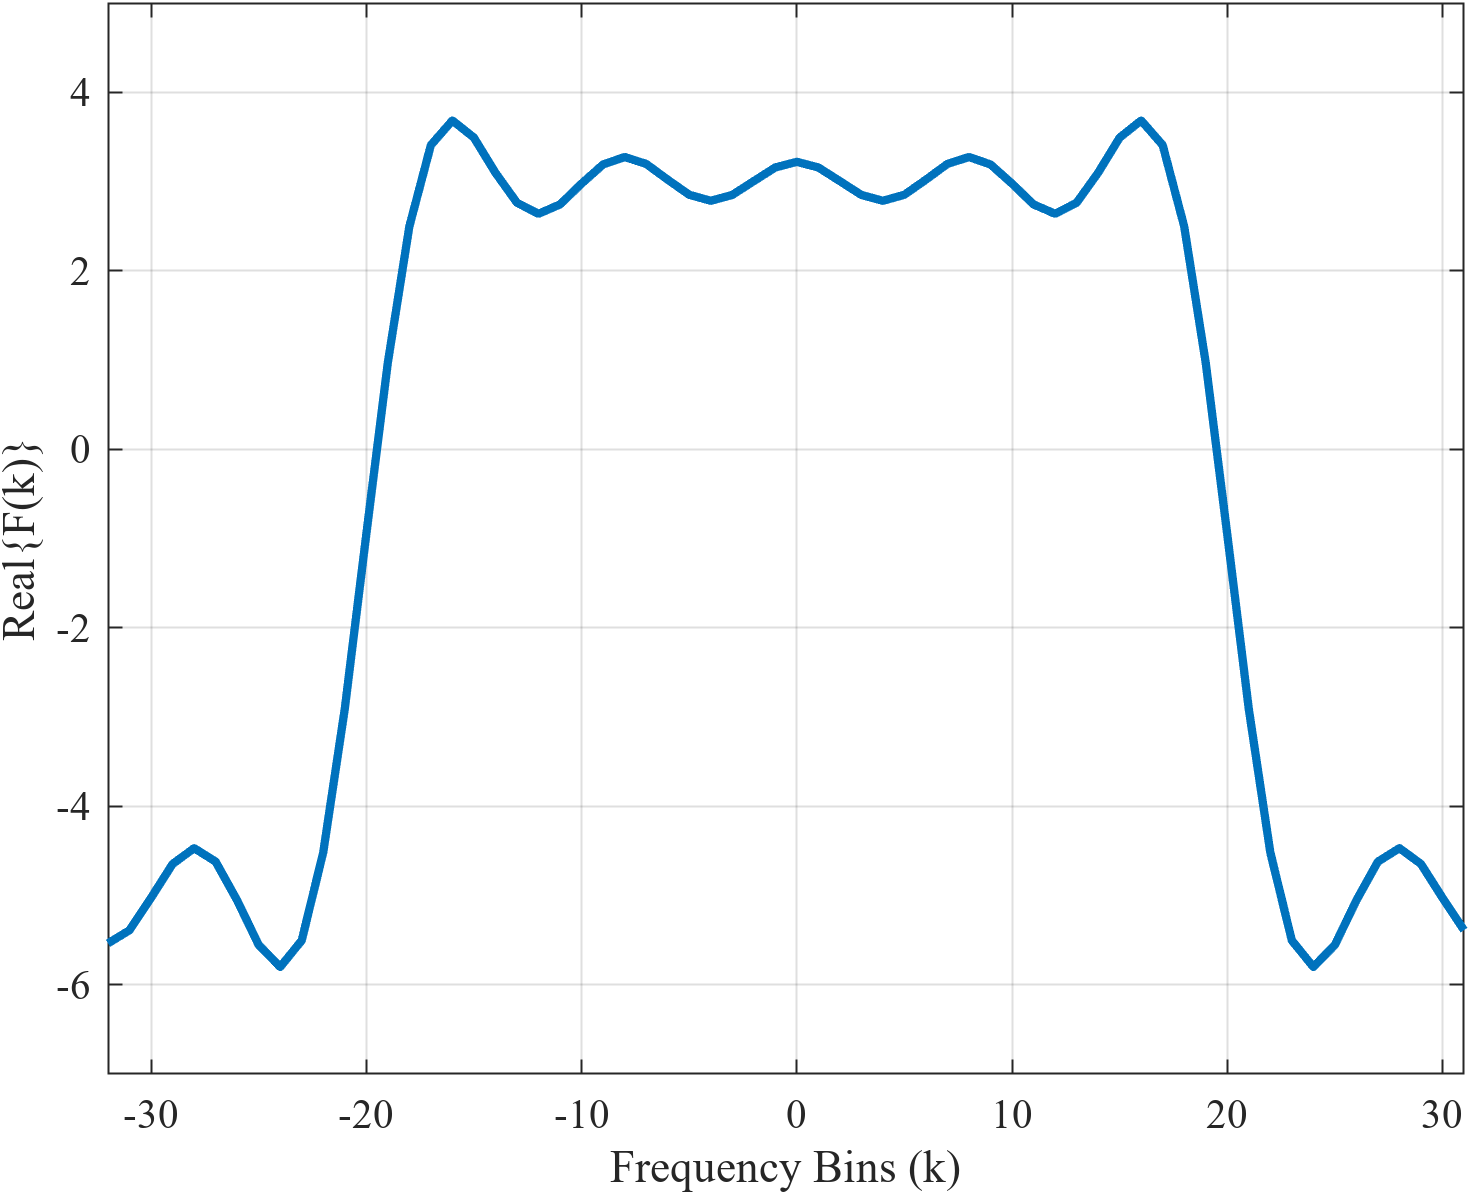
\includegraphics[width=0.8\textwidth]{DFT_64.png}
    \caption{64-point DFT of Fourier Coefficients}
\end{figure}


\newpage
\section*{Problem 6: Summary}
\begin{itemize}
    \item The Fourier series expansion resembles the periodic signal $f(t)$, but does not contain the discontinuities. To "match" the original signal, we would need to use more harmonics.
    \item The DTFT contains the same information as the Fourier series expansion, but is not periodic and is plotted on the interval $(-\pi, \pi)$.
    \item The 32-point and 64-point DFTs are similar to the DTFT, but are sampled at discrete intervals.
    \item The 32-point DFT has a lower frequency resolution than the 64-point DFT. I initially plotted these as bar graphs as the FFT is classically represented, but I kept the line plots for consistency with the DTFT. 
    \item The 32-point and 64-point DFTs demonstrate the effect of zero-padding on frequency resolution. The input to both contains the same information, so long as one does not conside the zeros as additional info. 
    \item The 64-point DFT has a higher resolution and is better able to represent the component frequencies.
    \item I spent more time on the \LaTeX{} than the actual homework, but I had fun and that's what matters.
\end{itemize}

\end{document}
